% !TEX root =../pfcTipoETSI.tex
%El anterior comando permite compilar este documento llamando al documento raíz
\chapter{Introducción}\LABCHAP{intro}
%\epigraph{}{}

%\lettrine[lraise=0.7, lines=1, loversize=-0.25]{E}{n}
\lettrine[lraise=-0.1, lines=2, loversize=0.2]{P}{r}oducir burbujas de tamaño micrométrico tiene, hoy día, numerosas aplicaciones que van más allá de aquellas destinadas a procesos  a escala de laboratorio. De hecho, el gran desarrollo y la diversidad de tecnologías desarrolladas en los últimos años han dado lugar a recientes revisiones del estado del arte que tratan con gran detalle tanto los fundamentos que sustentan la producción de microburbujas monodispersas como sus aplicaciones (véase~\cite{Rodriguez-Rodriguez2015b}). Tanto es así que el empleo de microburbujas tiene cabida en procesos de índole tan variada como el tratamiento de aguas, la industria alimentaria, y todo tipo de procesos médicos y farmacológicos, por citar algunos ejemplos. Así, para la obtención de imágenes por ultrasonidos, el uso de microburbujas como angentes de contraste ha demostrado arrojar unos excelentes resultados \cite{Ferrara2007,Kilbanov2006,Postema2005}. Por otro lado, las elevadas necesidades de aireación y el gran porcentaje que esta ocupa en el coste de operación de los biorreactores~\cite{Garcia-Ochoa2009,Rosso2008} hacen que el adecuado control del tamaño y la frecuencia de producción de las burbujas tenga un fuerte impacto en la eficiencia del proceso. 


Cuando se requiere el uso de microburbujas en aplicaciones como las mencionadas anteriormente, se dispone de tres variables que se desean controlar: el diámetro medio de las burbujas, $d_{b}$, la frecuencia de producción de estas, $f_{b}$ y el índice de polidispersión, PDI, ya que para considerar que la producción de microburbujas es monodispera estas tienen que tener un PDI por debajo del 5\%~\cite{Rodriguez-Rodriguez2015b}. Así, en el caso de la oxigenación de biorreactores, típicamente será necesario satisfacer la demanda de oxígeno de los microorganismos presentes, OUR~(\emph{Oxygen Uptake Rate}, de sus siglas en inglés), por lo que el ratio de transferencia de oxígeno~(\emph{Oxygen Transfer Rate}-OTR) puede ser el paso limitante en todo el proceso~\cite{Garcia-Ochoa2009}. El parámetro que controla el OTR es, dado un gradiente de concentración, el coeficiente de transferencia de masa, $k_{L}a$, el cual se encuentra direcamente afectado por la frecuencia y el diámetro de las burbujas. En efecto, el area específica de interfase, i.e. el area por unidad de volumen de las burbujas, depende de forma inversa del diámetro de las burbujas ($a = 6\phi/d_{b}$, con $\phi$ la fracción de gas en el medio). Por lo tanto, a menor diámetro de las burbujas mayor es el coeficiente de transferencia de transferencia de masa, lo que se traduce en última instancia en una reducción del caudal de aire requerido para satisfacer el OUR del cultivo, con el consiguiente ahorro que esta implica. Es por ello que el empleo de difusores de burbuja fina \cite{Sander2017,Rosso2008}, con diámetros 1-3~mm, o incluso de microburbujas \cite{Terasaka2011,Kawahara2009,Sadatomi2005}, con diámetros 10-500~$\mu$m, resulta esencial cuando se trata de aumentar la eficiencia del proceso de aireación; no obstante, también se ha reportado que la presencia de surfactantes y antiespumantes en el medio puede reducir críticamente el valor de dicho coeficiente en los casos en los que se favorece la coalescencia (véase~\cite{Garcia-Ochoa2005}), mientras que la presencia de una determinada concentración de sal (equivalente al lodo presente en las aguas no tratadas) puede inhibir precisamente esta coalescencia~\cite{Sander2017}. 

Como puede observarse, las exigencias de las industrias actuales, que requieren cada vez mayores frecuencias de producción y menores diámetros de las burbujas, conlleva que se hayan desarrollado diferentes tecnologías para poder conseguir una población monodispersa donde se pueda controlar tanto $d_{b}$ y $f_{b}$. Todas estas tecnologías emergentes emplean dispositivos microfluídicos de tamaño milimétrico y submilimétrico que, aunque puedan parecer muy similares entre sí, se fundamentan en principios físicos diferentes que conviene comprender~\cite{Rodriguez-Rodriguez2015b}. De este modo, el capítulo se estructura de la siguiente forma: en primer lugar, se realiza una descripción de las ecuaciones que gobiernan la dinámica de una burbuja que se produce en el seno de un líquido, después, se enumeran las diversas tecnologías que se han desarrollado y que se utilizan para generar una población monodispersa de microburbujas en los diferentes regímenes. En algunas de esta aplicaciones, el papel del gradiente de presión existente en el líquido exterior juega un papel fundamental que se describe con detalle en la \SEC{gradPres}. Finalmente, considerando las pequeñas geometrías empleadas en las tecnologías actuales y el rol determinante del gradiente de presión, se expondrán las ideas que han llevado al desarrollo del dispositivo que en este trabajo se estudia. 

\section{Fundamentos de la generación de burbujas}\LABSEC{fundamentos}

Lejos de lo que pudiera intuirse, la generación de burbujas es un proceso con importantes diferencias respecto al procceso de producción de gotas. En general, para generar gotas de radio $r_{d}$ a una frecuencia $f_{d}\sim U/r_{d}$, basta con injectar el líquido a través de un tubo de radio $r_{t}\sim r_{d}$ a una velocidad $U \gtrsim U_{c}$, con $U_{c} = \left[\sigma/\left(\rho g\right)\right]^{1/2}$ la velocidad capilar\footnote{Se remite al lector interesado en la rotura e inestabilidades de chorros líquidos a la excelente revisión~\cite{Eggers2008}}~\cite{Rodriguez-Rodriguez2015b}. 

Sin embargo, en el caso de la formación  de burbujas para estas condiciones, el comportamiento es diferente. Por un lado, en el caso de generación cuasiestática en el que $U \ll U_{c}$, el radio de la burbuja viene dado por el conocido \emph{radio de Fritz}, que resulta del balance de esfuerzos de tensión superficial con la fuerza de flotación, $r_{F}/r_{t} \sim \left[3/(2Bo)\right]^{1/3}$, con $Bo = \rho g r_{t}^{2}/\sigma$ el número de Bond, que mide la importancia relativa de los esfuerzos de tensión superficial frente a los esfuerzos de volumen  (gravedad/flotación). Sin embargo, si se desea reducir el diámetro de las burbujas o incrementar la frecuencia de producción aumentando la velocidad de inyección del gas a valores por encima de $U_{c}$, lejos de obtener un chorro de radio comparable al del injector, se obtienen (por encima de cierta velocidad) burbujas de volumen $V_{b} \propto \left(Q_{g}/g^{1/2}\right)^{6/5} > 4/3\pi r_{F}^{3}$~\cite{Rodriguez-Rodriguez2015b}, y lo que es más, si se sigue aumentando la velocidad, las burbujas cercanas entresí pueden coalescer, con lo que el diámetro final obtenido es mucho mayor~\cite{Higuera2006}. 

Para explicar estas diferencias entre ambos procesos, si se desprecian los efectos dinámicos del gas (ya que $\rho_{g}/\rho \gg 1$ y $\mu_{g}/\mu  \gg 1$), y se considera que la burbuja es prácticamente esférica, con una presión uniforme en su interior, la dinámica de la burbuja puede describirse a través de la ecuación de Rayleigh-Plesset.

\begin{equation}\LABEQ{rayleighPlesset}
\rho\left(R_{b}\ddot{R}_{b} + \dfrac{3}{2}\dot{R}_{b}^{2}\right) = \Delta p_{exit} - \dfrac{2\sigma}{R_{b}} - 4\mu \dfrac{\dot{R}_{b}}{R_{b}}
\end{equation}

Tal y como se puede observar en~\cite{Rodriguez-Rordiguez2015b}, para que el crecimiento de la burbuja y su posterior colapso tengan lugar, requiere que el término $\Delta p - 2\sigma/R_{b}$ cambie de positivo, valor que adquire en los primeros instantes mientras la burbuja se infla, a negativo, momento en el que las velocidades negativas cerca del inyector  la harán colapsar. La \EQ{rayleighPlesset} junto con la ecuación de continuidad

\begin{equation}\LABEQ{continuidad}
Q_{g} = \dfrac{\mathrm{d}V_{b}}{\mathrm{d}t} \simeq 4\pi R_{b}^{2} \dot{R}_{b}
\end{equation}

y el balance de cantidad de movimiento en la línea de gas\footnote{Nótese que no puede presuponerse, \textit{a priori}, la constancia del caudal, debido a las dos etapas bien diferenciadas que existen en el proceso de generación de burbujas.}

\begin{equation}\LABEQ{continuidad}
p_{0} - p_{exit} = \rho_{g}K\left(Re_{g}\right)\left[Q_{g}/\left(\pi r_{t}^{2}\right)\right]^{2}
\end{equation}

proporcionan el conjunto de ecuaciones necesario para describir sucintamente las tecnologías de la \SEC{tecnologias} y, con ellas, el diámetro y frecuencia de producción de las burbujas finalmente obtenidas. 
\begin{figure}[hbtp!]
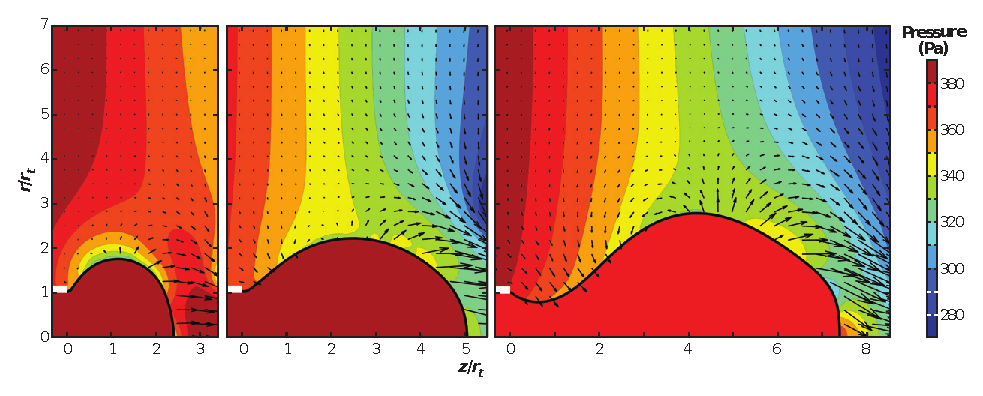
\includegraphics[width=\linewidth]{introduccion/figuras/esquemaBurbuja.eps}
\caption{Contornos de presión en las fases iniciales del proceso de formación de una burbuja para un número de Bond, $Bo = 0.245$. Cortesía de~\cite{Rodriguez-Rodriguez2015b}}
\LABFIG{esquemaBurbuja}
\end{figure}

Sintetizando una vez más las ideas expuestas en~\cite{Rodriguez-Rodriguez2015b}, el proceso de formación de una burbuja en una piscina en reposo puede esquematizarse en las siguientes etapas:

\begin{itemize}
\item En primer lugar, para satisfacer \EQ{continuidad}, el volumen de la burbuja debe aumentar, lo que provoca velocidades radiales en el líquido hacia fuera de la burbuja. 
\item La presión del gas en el interior de la burbuja es prácticamente uniforme, y debe adaptarse a la del líquido exterior en algún punto entre $z = 0$ (véase la \FIG{esquemaBurbuja}) y $z = 2R_{b}$, el cenit de la misma, supóngase en $z \sim R_{b}$. 
\item A medida que el radio de la burbuja aumenta, la punta de la burbuja se encuentra con una sobrepresión respecto al líquido exterior del orden de $\sim \rho g R_{b}$, lo que contribuye a que el gas acelere al líquido exterior, mientras que, en $z = 0$, es el líquido el que ejerce una sobrepresión sobre la base de la burbuja del orden de $\sim -\rho g R_{b}$, lo que conlleva que el líquido induzca velocidades hacia el interior de la burbuja. 
\end{itemize}

Por lo tanto, si nos ceñimos al caso no viscoso, la burbuja se desprenderá del inyector cuando la velocidad hacia adentro en $z = 0$, que surge del balance de \EQ{rayleighPlesset}, $\Delta p = p_{exit} - 2\sigma/R_{b} \sim \rho \dot{R}_{b}$ coincida con la velocidad hacia afuera impuesta por continuidad, $\sim Q_{g}/\left(4\pi R_{b}^{2}\right)$.

\begin{equation}\LABEQ{dbestimado}
\dfrac{Q_{g}}{R_{b}^{2}} \sim 	\sqrt{\dfrac{\Delta p}{\rho}} \sim \sqrt{g R_{b}} \Rightarrow d_{b} \sim \left(\dfrac{Q_{g}}{g^{1/2}}\right)^{2/5}
\end{equation}

siendo, finalmente, la frecuencia de producción 

\begin{equation}\LABEQ{fbestimado}
f_{b}\sim \dfrac{Q_{g}}{d_{b}^{3}} \sim	\left(\dfrac{g^{3}}{Q_{g}}\right)^{1/5}
\end{equation}

Así, aunque puede emplearse este sencillo método para producir burbujas simplemente inyectando gas en el seno de un líquido en reposo, la burbujas obtenidas poseen un diámetro significativamente mayor que el radio del inyector y con frecuencias que decrecen con el caudal, por lo que no resulta un método adecuado para satisfacer las demandas que las aplicaciones actuales requieren en lo que a diámetros y frecuencias se refiere\cite{Rodriguez-Rodriguez2015b}. Ello ha propiciado el desarrollo de tecnologías más sofisticadas basadas en dispositivos microfluídicos los cuales, en esencia, buscan aumentar el gradiente de presión (esto es, la gravedad efectiva) al que se ve sometida la gota en su proceso de generación. 




\section{Dispositivos para la generación de microburbujas}\LABSEC{tecnologias}

<<<<<<< HEAD
Una vez que se han descrito las ecuaciones necesarias para la compresión de los fundamentos de la generación de burbujas en el seno de un líquido, se está en disposición de enumerar y describir de forma sucinta las tecnologías más relevantes que, actualmente, se emplean para producir masivamente las mencionadas burbujas. Conviene recordar que las soluciones tecnológicas que aquí se presentan no son las únicas que permiten la producción de burbujas con tamaños submilimétricos; en efecto, en aplicaciones industriales como los reactores químicos, los esfuerzos de cortadura fruto de la turbulencia son los responsables de que la formación de burbujas que, aunque micrométricas y a grandes frecuencias, son generadas con un alto PDI~\cite{Rodriguez-Rodriguez2015b}.

De nuevo, tomando como referencia~\cite{Rodriguez-Rodriguez2015b}, respetará su estructura para presentar las tecnologías que a continuación se describen, no extendiénsose en exceso y pudiendo encontrar el lector una descripción más detallada tanto en el \textit{review} como en las referencias citadas en él. Así pues, en la \FIG{tecnologias}, se describen de forma esquemática los dispositivos más relevantes para la producción de burbujas actualmente. En la figura se pueden distinguir dos tipos principales de tecnologías: aquellas emplean una corriente de líquido para provocar el colapso de la corriente gaseosa para la formación de burbujas (\FIG{tecnologias}a-d) y aquellas que en las que se emplean ultrasonidos (\FIG{tecnologias}e-f). A su vez, de entre las primeras, se puede distinguir en aquellas en las que el líquido es inyectado en la misma dirección que la corriente gaseosa (\FIG{tecnologias}a-c) y aquellas en las que el líquido y el gas se encuentran de forma perpendicular (\FIG{tecnologias}d). Finalmente, la diferencia principal entre los dispositivos de \emph{flow-focussing} (\FIG{tecnologias}b-c), y los de \emph{coflow} es que en el primero se hace pasar ambos fluidos a través de un estrechamiento, lo que acelera colapso y permite generar burbujas más pequeñas~\cite{Rodriguez-Rodriguez2015b}.


\begin{figure}
\LABFIG{tecnologias}
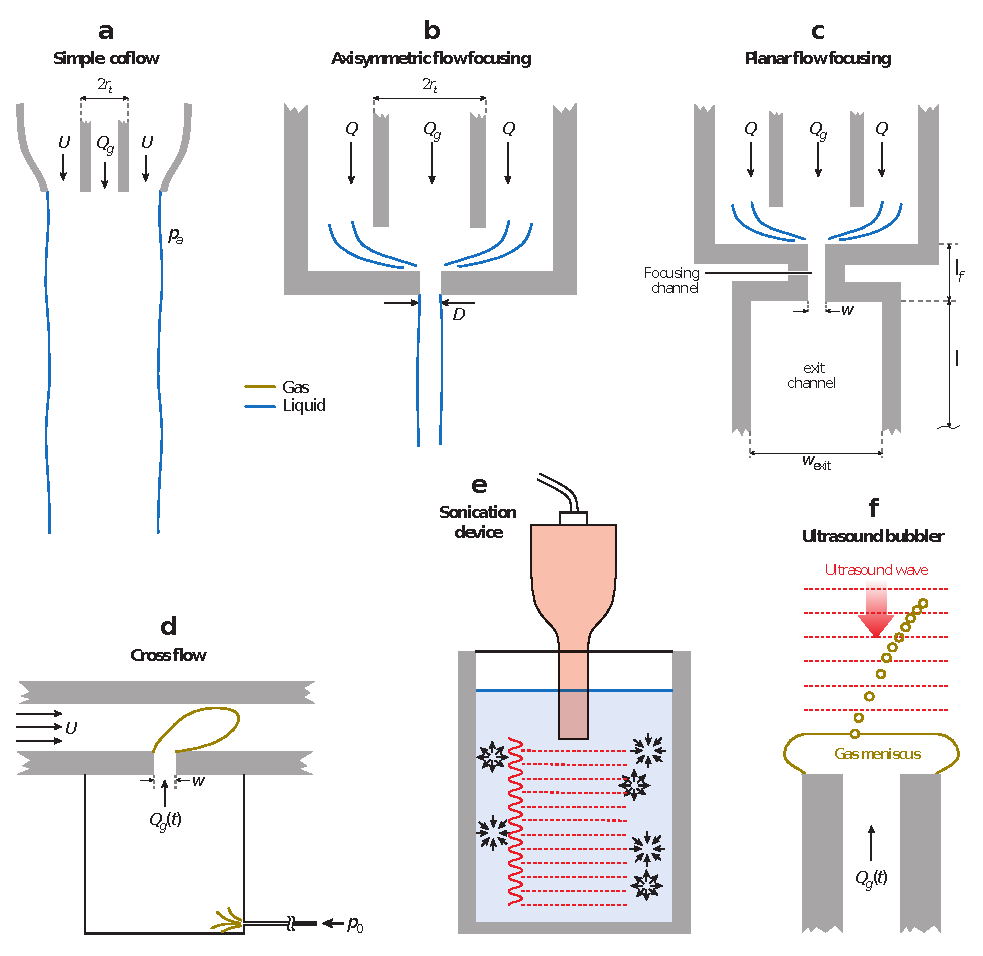
\includegraphics[scale=1]{figuras/tecnologias.eps}
\caption{Representación esquemática de los diferentes dispositivos que identifican la tecnología utilizada en la producción de burbujas monodispersas. Figura adaptada de~\cite{Rodriguez-Rodriguez2015b}.}
\end{figure}

\subsection{Dispositivos de Coflow}\LABSSEC{coflow}

Un dispositivo de tipo coflow es aquél como el mostrado en la \FIG{tecnologias}a, donde la corriente gaseosa y la de líquido son inyectadas en la misma dirección y de forma libre. Las condiciones en las que usualmente se opera este tipo de dispositivos son aquellas en las que el número de Reynolds y Webber son tales que $Re = \rho U r_{t}/\mu \gg 1$ y $We = \rho U^{2} r_{t}/ \sigma$. Bajo estas condiciones, las frecuencias de producción, $f_{b}$ y los diámetros equivalentes de las burbujas obtenidas, $d_{b} = \left[\left(6Q_{g}\right)/\left(\pi f_{b}\right)\right]^{\left(1/3\right)} $, dependen sólo del ratio de velocidades gas-líquido, $U_{g}/U$, y del ratio $r_{t}/U$. Además, en los casos bajo consideración donde $We \gg 1$, el líquido exterior impone la velocidad a la que la interfase es transportada, con lo que se previene la coalescencia ya que las burbujas son transportadas a la velocidad del líquido%PONER AQUI CITA DEL ARTÍCULO DE A.SEVILLA
. Precisamente, en una operación normal con este tipo de dispositivos, la velocidad del gas suele ser mayor que la del líquido, con lo que las burbujas son generadas cerca de la punta del inyector. 

=======
Una vez se ha descrito de forma muy resumida cómo es y qué factores conforman el proceso de formación de burbujas, y teniendo en cuenta las conclusiones finales extraídas de la \SEC{
>>>>>>> 686481c8352b2afedea906ec88ac2357e9cfe57a

\section{Influencia del gradiente de presión. Analogía aerodinámica}\LABSEC{gradPress}
